\subsection{Decoding the Frequency Limits of Your Digital Oscilloscope!}

\begin{tcolorbox}[colback=gray!10, colframe=black, title=E4A01]
Which of the following limits the highest frequency signal that can be accurately displayed on a digital oscilloscope?
\begin{enumerate}[label=\Alph*.]
    \item \textbf{A} Sampling rate of the analog-to-digital converter
    \item B Analog-to-digital converter reference frequency
    \item C Q of the circuit
    \item D All these choices are correct
\end{enumerate} \end{tcolorbox}

\subsubsection{Correct Answer}


\subsubsection{Related Concepts}
To understand why the sampling rate of the analog-to-digital converter (ADC) limits the highest frequency signal displayed on a digital oscilloscope, we need to consider the Nyquist-Shannon sampling theorem. This theorem states that in order to accurately capture a signal without aliasing, it must be sampled at least twice the highest frequency present in the signal.

\subsubsection{Calculation}
Let \( f_{max} \) be the maximum frequency of the signal and \( f_s \) be the sampling frequency of the ADC. According to the Nyquist theorem, the following must hold true:

\begin{equation}
f_s \geq 2f_{max}
\end{equation}

Rearranging for \( f_{max} \):

\begin{equation}
f_{max} \leq \frac{f_s}{2}
\end{equation}

For example, if an oscilloscope has an ADC with a sampling rate of 1 GHz, the maximum frequency that can be accurately displayed without aliasing would be:

\begin{equation}
f_{max} \leq \frac{1 \text{ GHz}}{2} = 500 \text{ MHz}
\end{equation}

This implies that signals of frequency higher than 500 MHz would not be accurately represented, and potential aliasing could occur.

\subsubsection{Diagram}
\begin{center}
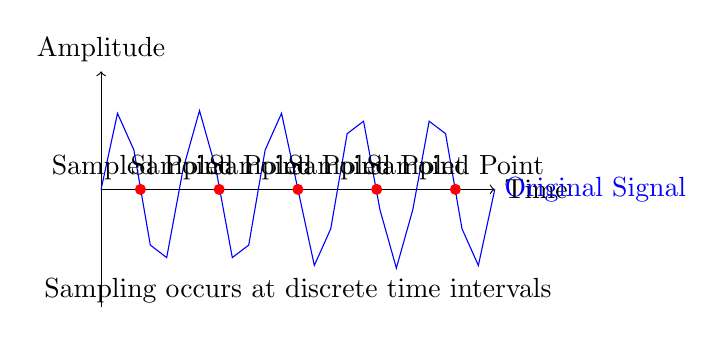
\begin{tikzpicture}
    \draw[->] (0,0) -- (5,0) node[right] {Time};
    \draw[->] (0,-1.5) -- (0,1.5) node[above] {Amplitude};
    
    % Signal
    \draw[blue] plot[domain=0:5] (\x,{sin(2*pi*1*\x r)}) node[right] {Original Signal};
    
    % Sampling points
    \foreach \x in {0.5, 1.5, 2.5, 3.5, 4.5} {
        \fill[red] (\x, {sin(2*pi*1*\x r)}) circle (2pt);
    }
    
    % Vertical line to show sampling
    \foreach \x in {0.5, 1.5, 2.5, 3.5, 4.5} {
        \draw[dashed] (\x, 0) -- (\x, {sin(2*pi*1*\x r)}) node[above] {Sampled Point};
    }
    
    \node[below] at (2.5,-1) {Sampling occurs at discrete time intervals};
    
\end{tikzpicture}
\end{center}
